%%%%%%%%%%%%%%%%%%%%%%%%%%%%%%%%%%%%%%%%%
% Beamer Presentation
% LaTeX Template
% Version 1.0 (10/11/12)
%
% This template has been downloaded from:
% http://www.LaTeXTemplates.com
%
% License:
% CC BY-NC-SA 3.0 (http://creativecommons.org/licenses/by-nc-sa/3.0/)
%
%%%%%%%%%%%%%%%%%%%%%%%%%%%%%%%%%%%%%%%%%

%----------------------------------------------------------------------------------------
%	PACKAGES AND THEMES
%----------------------------------------------------------------------------------------

\documentclass{beamer}

\usepackage{listings}
\lstset{ %
  basicstyle=\fontsize{9}{11}\ttfamily,
  backgroundcolor=\color{white},   % choose the background color; you must add \usepackage{color} or \usepackage{xcolor}; should come as last argument
  breakatwhitespace=false,         % sets if automatic breaks should only happen at whitespace
  breaklines=true,                 % sets automatic line breaking
  captionpos=b,                    % sets the caption-position to bottom
  commentstyle=\color{codegreen},    % comment style
  frame=tb,	                       % adds a frame around the code
  rulecolor=\color{black},         % if not set, the frame-color may be changed on line-breaks within not-black text (e.g. comments (green here))
  showspaces=false,                % show spaces everywhere adding particular underscores; it overrides 'showstringspaces'
  showstringspaces=false,          % underline spaces within strings only
  showtabs=false,                  % show tabs within strings adding particular underscores
  tabsize=2,	                     % sets default tabsize to 2 spaces
}



\mode<presentation> {

% The Beamer class comes with a number of default slide themes
% which change the colors and layouts of slides. Below this is a list
% of all the themes, uncomment each in turn to see what they look like.

%\usetheme{default}
%\usetheme{AnnArbor}
%\usetheme{Antibes}
%\usetheme{Bergen}
%\usetheme{Berkeley}
%\usetheme{Berlin}
%\usetheme{Boadilla}
%\usetheme{CambridgeUS}
%\usetheme{Copenhagen}
%\usetheme{Darmstadt}
%\usetheme{Dresden}
%\usetheme{Frankfurt}
%\usetheme{Goettingen}
%\usetheme{Hannover}
%\usetheme{Ilmenau}
%\usetheme{JuanLesPins}
%\usetheme{Luebeck}
\usetheme{Madrid}
%\usetheme{Malmoe}
%\usetheme{Marburg}
%\usetheme{Montpellier}
%\usetheme{PaloAlto}
%\usetheme{Pittsburgh}
%\usetheme{Rochester}
%\usetheme{Singapore}
%\usetheme{Szeged}
%\usetheme{Warsaw}

% As well as themes, the Beamer class has a number of color themes
% for any slide theme. Uncomment each of these in turn to see how it
% changes the colors of your current slide theme.

%\usecolortheme{albatross}
%\usecolortheme{beaver}
%\usecolortheme{beetle}
%\usecolortheme{crane}
%\usecolortheme{dolphin}
%\usecolortheme{dove}
%\usecolortheme{fly}
%\usecolortheme{lily}
%\usecolortheme{orchid}
%\usecolortheme{rose}
%\usecolortheme{seagull}
%\usecolortheme{seahorse}
%\usecolortheme{whale}
%\usecolortheme{wolverine}

%\setbeamertemplate{footline} % To remove the footer line in all slides uncomment this line
%\setbeamertemplate{footline}[page number] % To replace the footer line in all slides with a simple slide count uncomment this line

%\setbeamertemplate{navigation symbols}{} % To remove the navigation symbols from the bottom of all slides uncomment this line
}

\usepackage{graphicx} % Allows including images
\usepackage{booktabs} % Allows the use of \toprule, \midrule and \bottomrule in tables

%----------------------------------------------------------------------------------------
%	TITLE PAGE
%----------------------------------------------------------------------------------------

\title[Short title]{
Emulate the \texttt{persp()} plot and \texttt{filled.contour()} plot on \textbf{gridGraphics}
} % The short title appears at the bottom of every slide, the full title is only on the title page

\author{Zhijian Wen} % Your name
\institute[UCLA] % Your institution as it will appear on the bottom of every slide, may be shorthand to save space
{
University of Auckland \\ % Your institution for the title page
\medskip
\textit{jwen246@aucklanduni.ac.nz} % Your email address
}
\date{\today} % Date, can be changed to a custom date

\usepackage{Sweave}
\begin{document}
\Sconcordance{concordance:presentation.tex:presentation.Rnw:%
1 106 1 1 0 49 1 1 7 2 0 2 1 3 0 1 2 10 1 1 22 1 0 1 1 3 0 1 2 9 1 1 2 %
1 0 1 1 3 0 1 2 29 1 1 8 151 1 1 12 202 1 1 41 66 1 1 88 76 1}


\begin{frame}
\titlepage % Print the title page as the first slide
\end{frame}

\begin{frame}
\frametitle{Overview} % Table of contents slide, comment this block out to remove it
\tableofcontents % Throughout your presentation, if you choose to use \section{} and \subsection{} commands, these will automatically be printed on this slide as an overview of your presentation
\end{frame}

%----------------------------------------------------------------------------------------
%	PRESENTATION SLIDES
%----------------------------------------------------------------------------------------

%------------------------------------------------
\section{What is \texttt{gridGraphics}}

\subsection{Introduction} 
\begin{frame}
\frametitle{Introduction}
\begin{block}{What is \textbf{gridGraphics}...}
\textbf{gridGraphics} is the \textbf{R} package that convert \textbf{graphics}-plot to \textbf{grid}-plot.
\end{block}

\end{frame}

%------------------------------------------------

\begin{frame}[fragile]
\frametitle{Example}
\begin{Schunk}
\begin{Sinput}
> plot(cars$dist ~ cars$speed, pch = 16, 
+      col = 'orange', main = 'Distance vs Speed')
> library(gridGraphics)
> grid.echo()
\end{Sinput}
\end{Schunk}
\begin{center}
  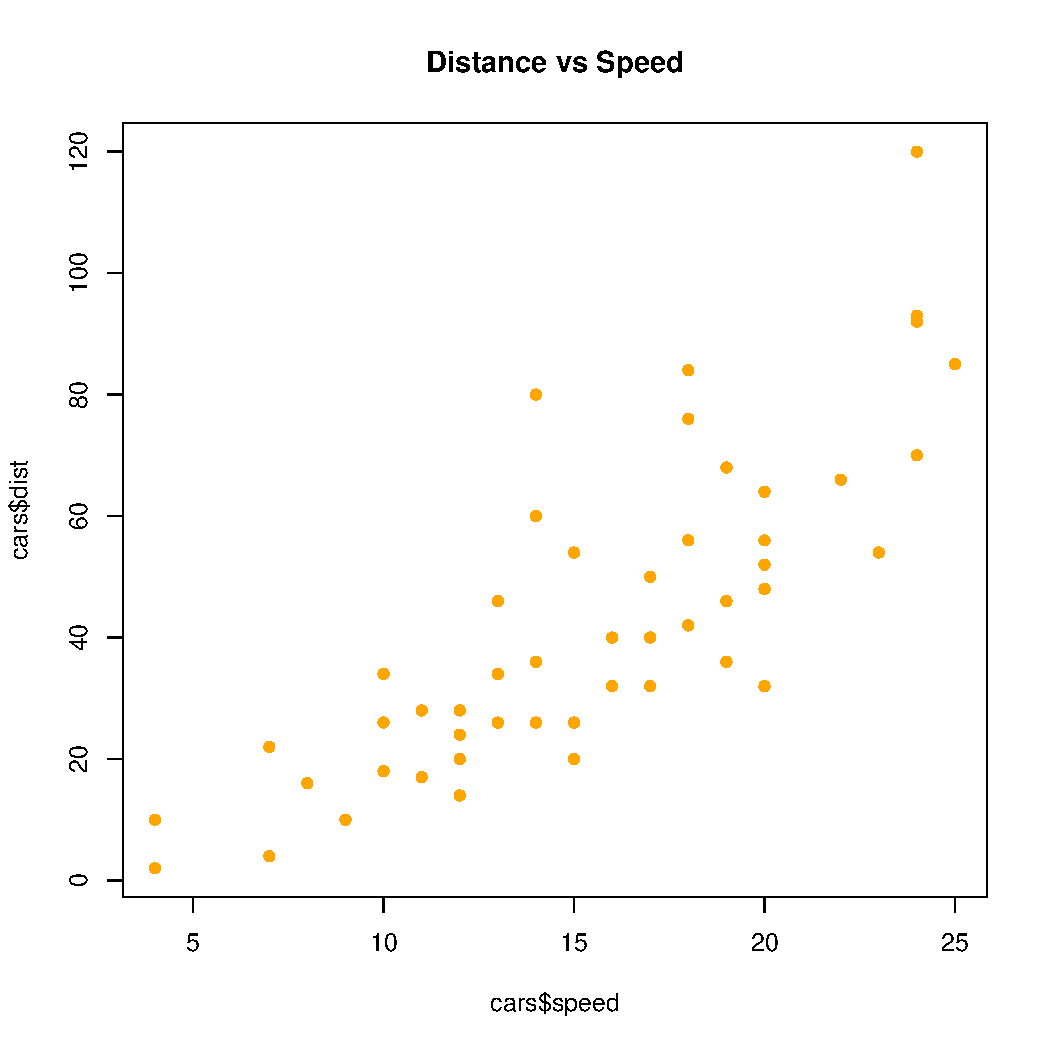
\includegraphics[height = 5.5cm, width = 5.5cm]{plot/intro_1.pdf}
  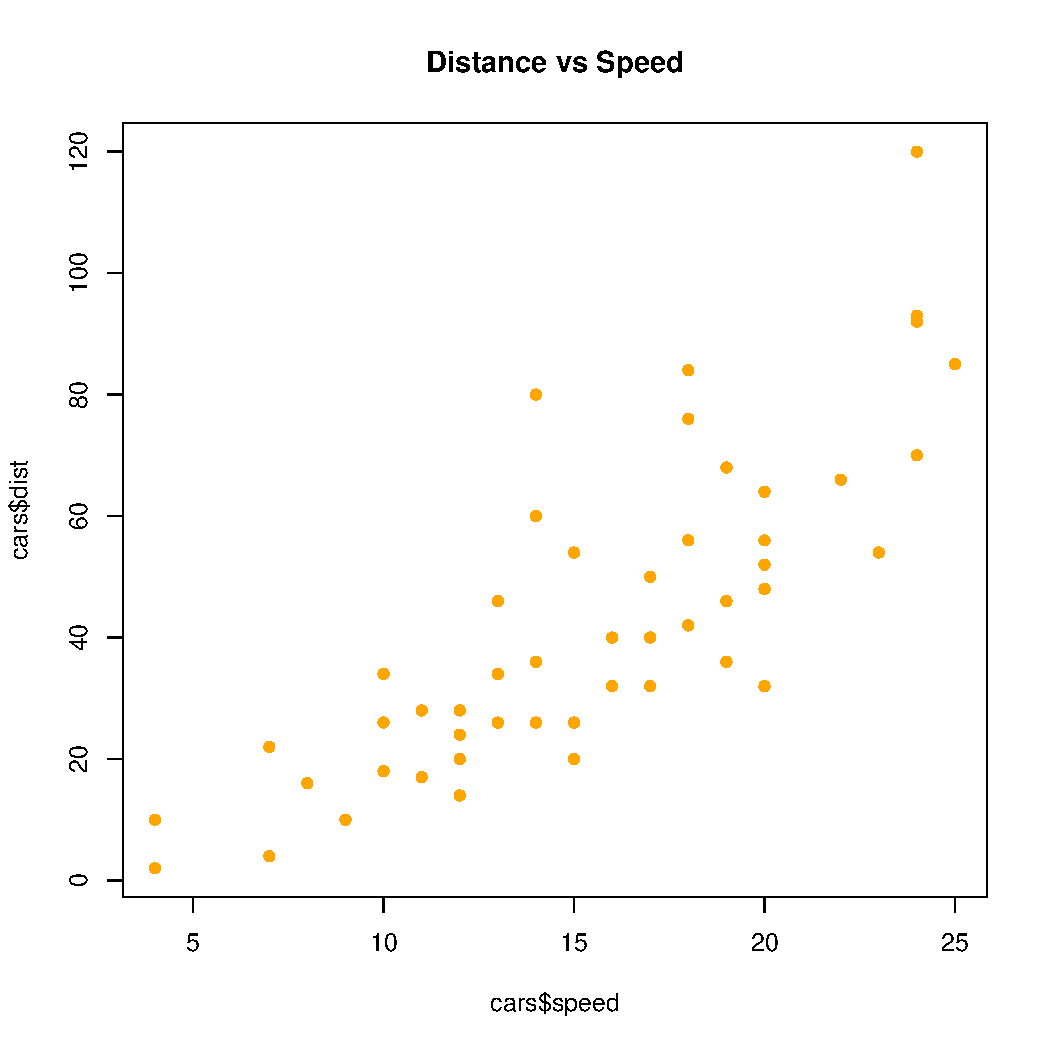
\includegraphics[height = 5.5cm, width = 5.5cm]{plot/intro_2.pdf}
\end{center}
\end{frame}

%------------------------------------------------

\begin{frame}[fragile]
\frametitle{The problem}
\begin{Schunk}
\begin{Sinput}
> x = y = seq(-4*pi, 4*pi, len = 27)
> r = sqrt(outer(x^2, y^2, "+"))
> filled.contour(cos(r^2)*exp(-r/(2*pi)))
> grid.echo()
\end{Sinput}
\end{Schunk}
\begin{center}
  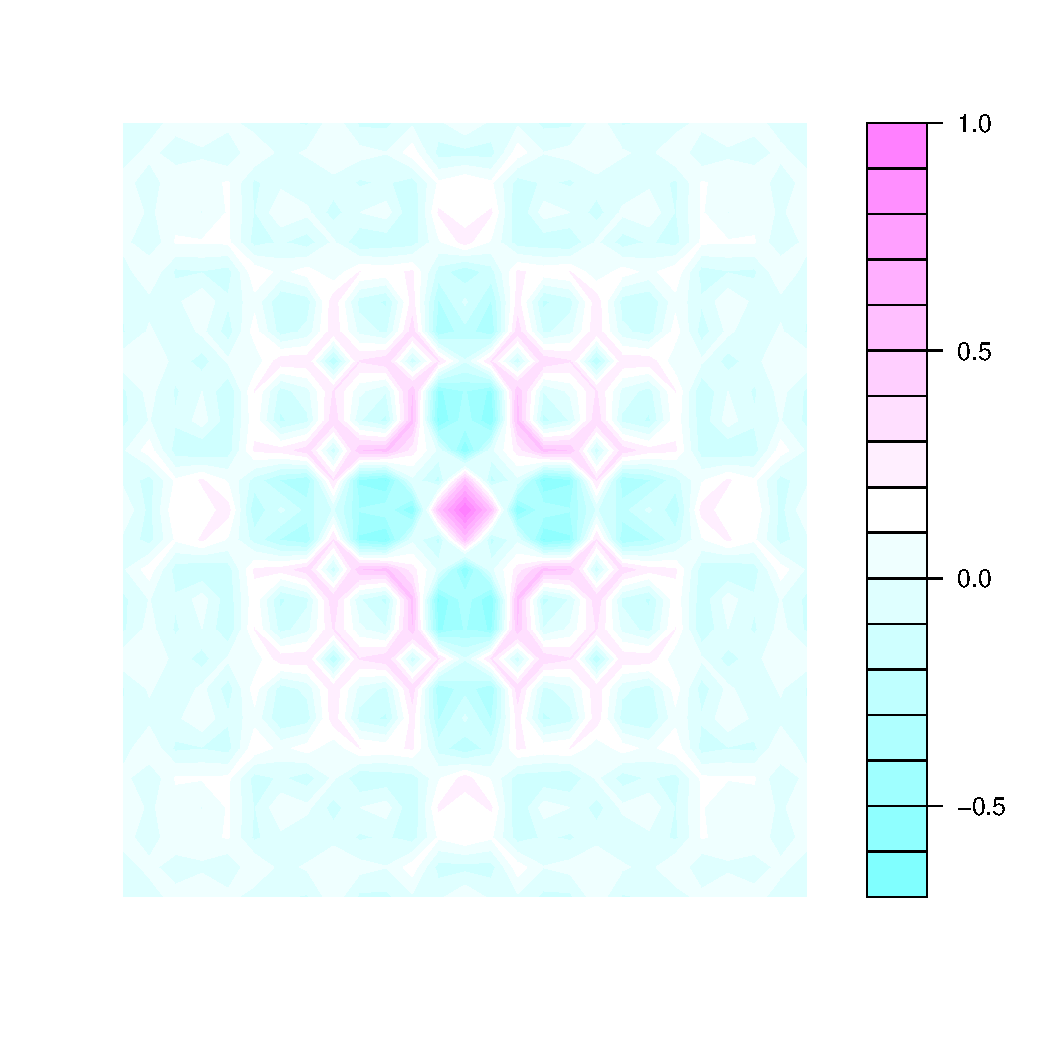
\includegraphics[height = 5.5cm, width = 5.5cm]{plot/report_fill_1}
  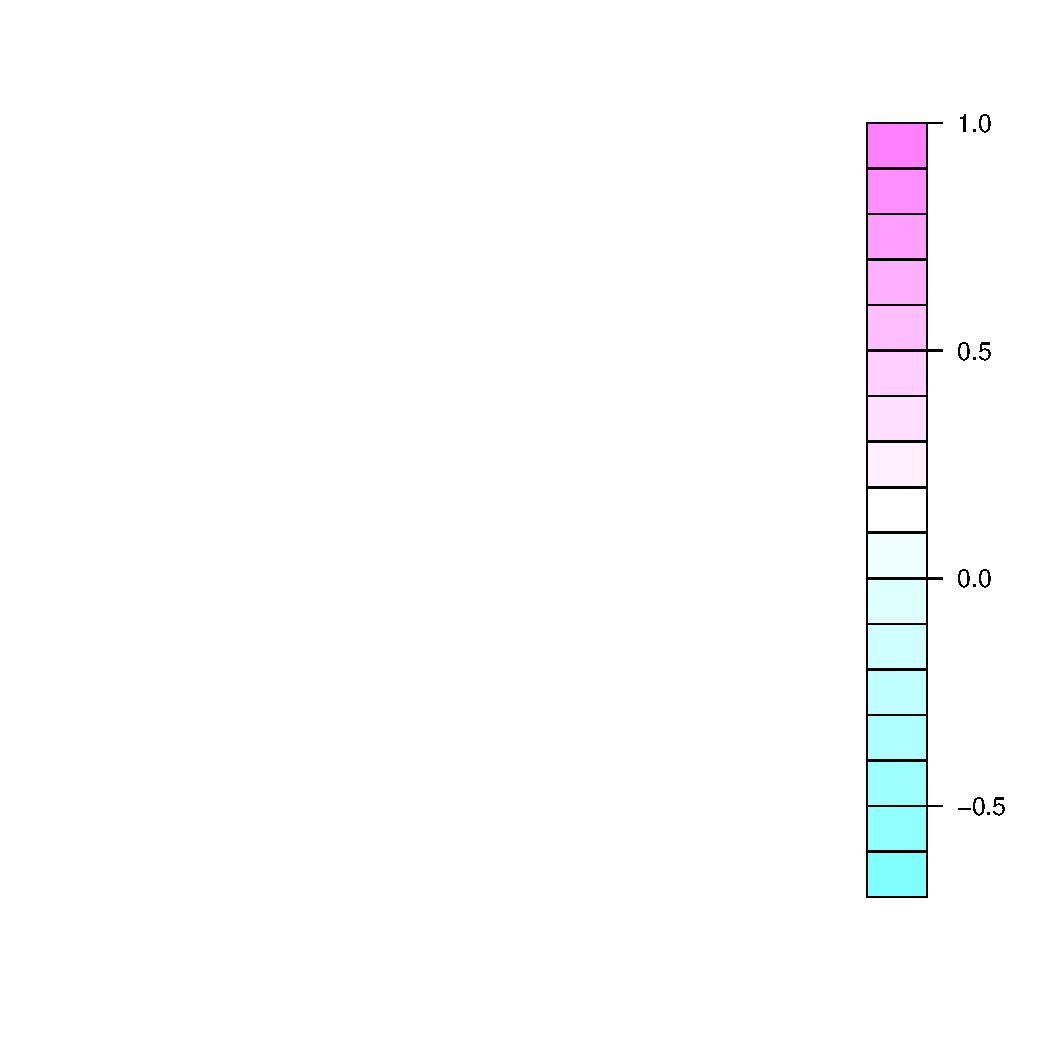
\includegraphics[height = 5.5cm, width = 5.5cm]{plot/report_fill_2}
\end{center}

\end{frame}

%------------------------------------------------

\begin{frame}[fragile]
\frametitle{How \textbf{gridGraphics} works?}


\begin{lstlisting}[language = R]
x <- recordPlot()
unlist(lapply(x[[1]], function(y) y[[2]][[1]]$name))
\end{lstlisting}

\begin{columns}[c]
\column{0.4\textwidth}
\begin{lstlisting}[language = R]
"C_plot_new"    
"palette2"      
"C_plot_window" 
"C_plotXY"      
"C_axis"        
"C_axis"       
"C_box"         
"C_title"    
\end{lstlisting}


\column{0.4\textwidth}
\begin{center}
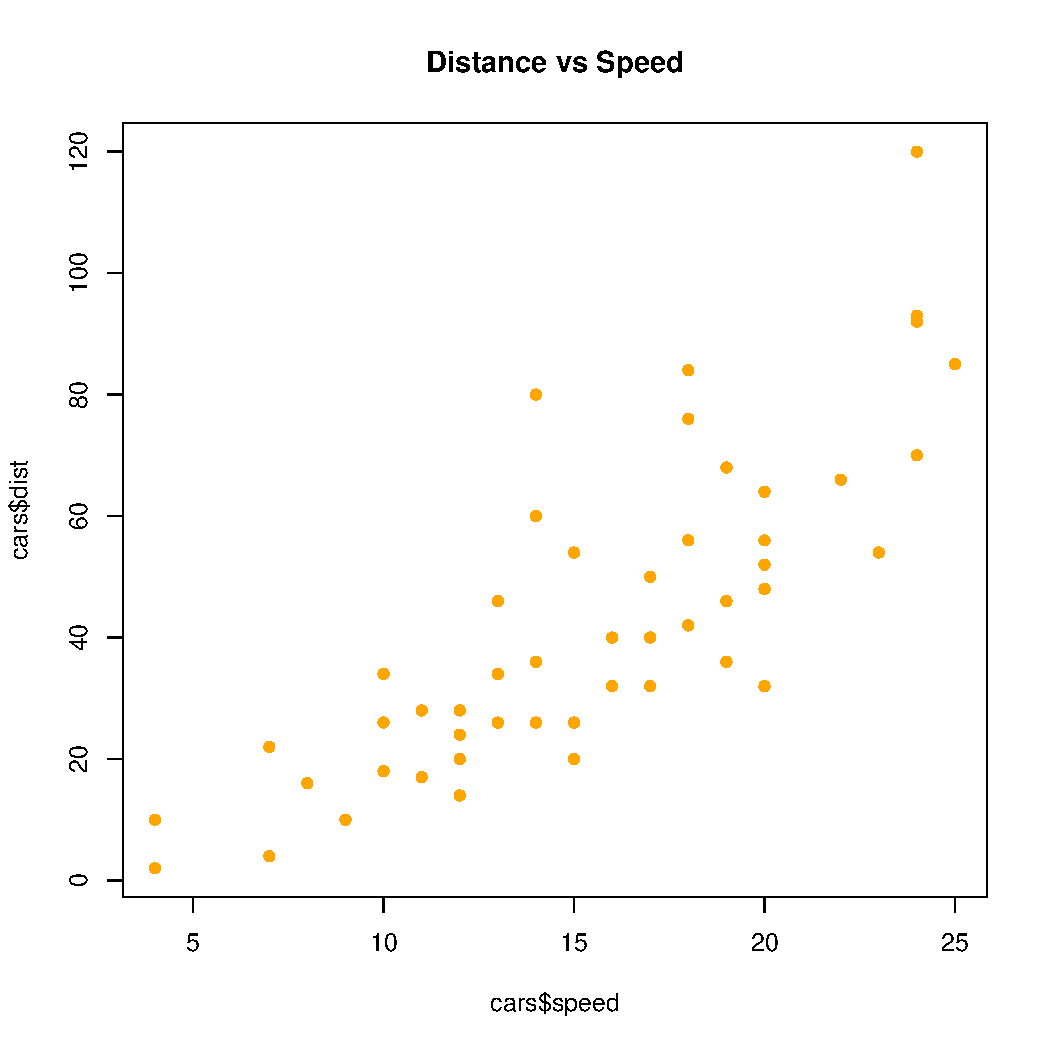
\includegraphics[height = 5.5cm, width = 5.5cm]{plot/intro_1.pdf}
\end{center}

\end{columns}

\end{frame}


%------------------------------------------------

\begin{frame}[fragile]
\frametitle{How \textbf{gridGraphics} works?}
\begin{Schunk}
\begin{Sinput}
> Sinc_Curve()
\end{Sinput}
\end{Schunk}
\begin{center}
  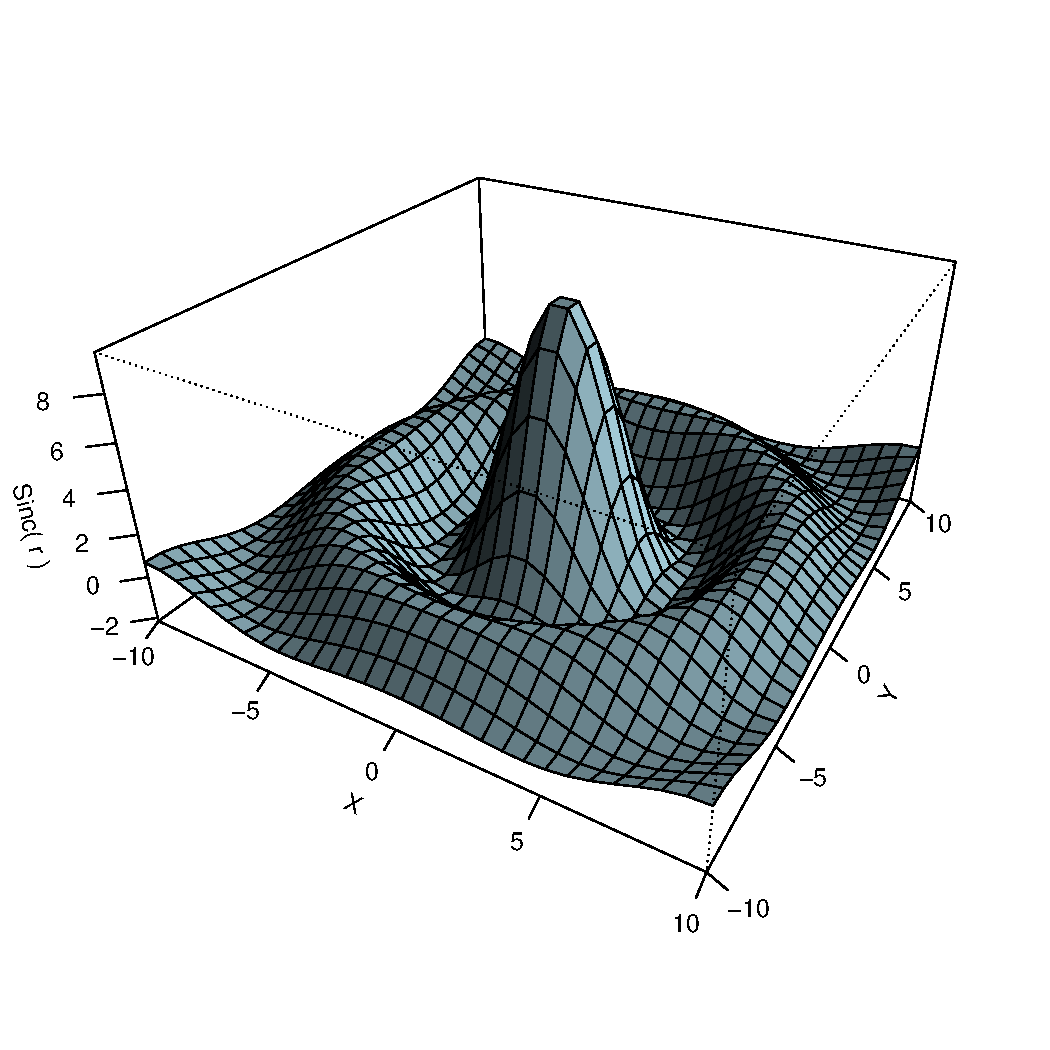
\includegraphics[height = 7.5cm, width = 7.5cm]{plot/persp_1}
\end{center}



\end{frame}

%------------------------------------------------

\begin{frame}[fragile]
\frametitle{How \textbf{gridGraphics} works?}
\begin{Schunk}
\begin{Sinput}
> x <- recordPlot()
> lapply(x[[1]], function(y) y[[2]][[1]]$name)
\end{Sinput}
\begin{Soutput}
[[1]]
[1] "C_plot_new"

[[2]]
[1] "palette2"

[[3]]
[1] "C_persp"
\end{Soutput}
\end{Schunk}
\begin{center}
\end{center}

\end{frame}



\begin{block}{Block 1}
Lorem ipsum dolor sit amet, consectetur adipiscing elit. Integer lectus nisl, ultricies in feugiat rutrum, porttitor sit amet augue. Aliquam ut tortor mauris. Sed volutpat ante purus, quis accumsan dolor.
\end{block}

\begin{block}{Block 2}
Pellentesque sed tellus purus. Class aptent taciti sociosqu ad litora torquent per conubia nostra, per inceptos himenaeos. Vestibulum quis magna at risus dictum tempor eu vitae velit.
\end{block}

\begin{block}{Block 3}
Suspendisse tincidunt sagittis gravida. Curabitur condimentum, enim sed venenatis rutrum, ipsum neque consectetur orci, sed blandit justo nisi ac lacus.
\end{block}
\end{frame}

%------------------------------------------------

\begin{frame}
\frametitle{Multiple Columns}
\begin{columns}[c] % The "c" option specifies centered vertical alignment while the "t" option is used for top vertical alignment

\column{.45\textwidth} % Left column and width
\textbf{Heading}
\begin{enumerate}
\item Statement
\item Explanation
\item Example
\end{enumerate}

\column{.5\textwidth} % Right column and width
Lorem ipsum dolor sit amet, consectetur adipiscing elit. Integer lectus nisl, ultricies in feugiat rutrum, porttitor sit amet augue. Aliquam ut tortor mauris. Sed volutpat ante purus, quis accumsan dolor.

\end{columns}
\end{frame}

%------------------------------------------------
\section{Second Section}
%------------------------------------------------

\begin{frame}
\frametitle{Table}
\begin{table}
\begin{tabular}{l l l}
\toprule
\textbf{Treatments} & \textbf{Response 1} & \textbf{Response 2}\\
\midrule
Treatment 1 & 0.0003262 & 0.562 \\
Treatment 2 & 0.0015681 & 0.910 \\
Treatment 3 & 0.0009271 & 0.296 \\
\bottomrule
\end{tabular}
\caption{Table caption}
\end{table}
\end{frame}

%------------------------------------------------

\begin{frame}
\frametitle{Theorem}
\begin{theorem}[Mass--energy equivalence]
$E = mc^2$
\end{theorem}
\end{frame}

%------------------------------------------------

\begin{frame}[fragile] % Need to use the fragile option when verbatim is used in the slide
\frametitle{Verbatim}
\begin{example}[Theorem Slide Code]
\begin{verbatim}
\begin{frame}
\frametitle{Theorem}
\begin{theorem}[Mass--energy equivalence]
$E = mc^2$
\end{theorem}
\end{frame}\end{verbatim}
\end{example}
\end{frame}

%------------------------------------------------

\begin{frame}
\frametitle{Figure}
Uncomment the code on this slide to include your own image from the same directory as the template .TeX file.
%\begin{figure}
%\includegraphics[width=0.8\linewidth]{test}
%\end{figure}
\end{frame}

%------------------------------------------------

\begin{frame}[fragile] % Need to use the fragile option when verbatim is used in the slide
\frametitle{Citation}
An example of the \verb|\cite| command to cite within the presentation:\\~

This statement requires citation \cite{p1}.
\end{frame}

%------------------------------------------------

\begin{frame}
\frametitle{References}
\footnotesize{
\begin{thebibliography}{99} % Beamer does not support BibTeX so references must be inserted manually as below
\bibitem[Smith, 2012]{p1} John Smith (2012)
\newblock Title of the publication
\newblock \emph{Journal Name} 12(3), 45 -- 678.
\end{thebibliography}
}
\end{frame}

%------------------------------------------------

\begin{frame}
\Huge{\centerline{The End}}
\end{frame}

%----------------------------------------------------------------------------------------

\end{document}
